\chapter{Solution}
\label{cha:solution}

\sloppy

This chapter will present \texttt{xmlet}, its different components and how they interact between them. Generating a Java \textit{fluent interface} based on a \ac{XSD} file includes two distinct tasks:

\begin{enumerate}
	\item Parsing the information from the \ac{XSD} file;
	\item Generating the \textit{fluent interface} classes based on the resulting information of the previous task.
\end{enumerate}

\noindent
Those tasks are encompassed by two different projects, \hyperref[sec:xsdparser]{XsdParser}, presented in Section \ref{sec:xsdparser}, and \hyperref[sec:xsdasm]{XsdAsm}, presented in Section \ref{sec:xsdasm}. In this case the XsdAsm has a dependency to XsdParser.

\noindent
The main use case of \texttt{xmlet} is the generation of a Java \ac{DSL} for \ac{HTML}. To that end, the HtmlApi, presented in Section \ref{sec:htmlapi}, specifies how the XsdAsm project can be used, specifically using the \ac{HTML}5 \ac{XSD} file, to generate the Java \ac{HTML} \textit{fluent interface}.

\noindent
Finally, the HtmlFlow 3 is responsible for establishing the output of a concrete HtmlApi usage. Some additional remarks regarding changes on the HtmlFlow library will be provided in Section \ref{sec:htmlflow3}.

\section{XsdParser} % (fold)
\label{sec:xsdparser}

XsdParser is a library that parses a \ac{XSD} file into a list of Java objects. Each different \ac{XSD} tag has a corresponding Java class and the  attributes of a given \ac{XSD} type are represented as fields of that class. All these classes derive from the same abstract class, \texttt{XsdAbstractElement}. All Java representations of the \ac{XSD} elements follow the schema definition for \ac{XSD} elements, referred in Section \ref{sec:xsd}. For example, the \texttt{xsd:annotation} tag only allows \texttt{xsd:appinfo} and \texttt{xsd:documentation} as children nodes, and can also have an attribute named \texttt{id}, therefore XsdParser has the following class as shown in Listing \ref{lst:xsdannotationexample}.

\bigskip

\lstset{language=java, morekeywords={XsdAppInfo, XsdDocumentation, ArrayList, List, XsdAbstractElement, XsdAnnotation, String}}

\begin{minipage}{\linewidth}
\begin{lstlisting}[caption={Simplified Version of the Generated XsdAnnotation Class}, label={lst:xsdannotationexample}]
public class XsdAnnotation extends XsdAbstractElement {

    private String id;
    private List<XsdAppInfo> appInfoList = new ArrayList<>();
    private List<XsdDocumentation> documentations = new ArrayList<>();
    
    // (...)
}
\end{lstlisting}
\end{minipage}

\subsection{Parsing Strategy}
\label{sec:parsingstrategy}

The first step of this library is handling the \ac{XSD} file. The Java language has no built in library that parses \ac{XSD} files, so we needed to look for other options. The main libraries found that address this problem were \ac{DOM} and \ac{SAX}. After evaluating the pros and cons of those libraries the choice ended up being \ac{DOM}, since a \ac{XSD} file is a tree of \ac{XML} elements. This choice was based mostly on the fact that \ac{SAX} is an event driven parser and \ac{DOM} is a tree based parser, which is more adequate for the present issue. \ac{DOM} is a library that maps \ac{HTML}, \ac{XHTML} and \ac{XML} files into a tree structure composed by multiple elements, also named nodes. This is exactly what XsdParser requires to obtain all the information from the \ac{XSD} files, which is described in \ac{XML}. 

\noindent
This means that XsdParser uses \ac{DOM} to parse the \ac{XSD} file and obtain its root element, a \texttt{xs:schema} node, performing a single read on the \ac{XSD} file, avoiding multiple reads, which are less efficient (Listing \ref{lst:nodelist}). 

\bigskip

\lstset{language=java, morekeywords={Document, DocumentBuilderFactory, DocumentBuilder, IOException, SAXException, ParserConfigurationException, Node, String}}

\begin{minipage}{\linewidth}
\begin{lstlisting}[caption={DOM Document Parsing}, label={lst:nodelist}]
private Node getSchemaNode(String filePath) 
    throws IOException, SAXException, ParserConfigurationException {
    DocumentBuilderFactory dbFactory =                                                              
                                DocumentBuilderFactory.newInstance();
    DocumentBuilder dBuilder = dbFactory.newDocumentBuilder();
    Document doc = dBuilder.parse(xsdFile);   //Parses the XSD file.

    // Obtains the first node of the document, which 
    // should be the xs:schema node.
    return doc.getFirstChild();
}
\end{lstlisting}
\end{minipage}

\noindent
After obtaining the root node of the \ac{XSD} file the XsdParser verifies if that node is a \texttt{XsdSchema} node as shown in Listing \ref{lst:nodeparsingprocess}. If that is the case it proceeds by performing the \texttt{parse} function of the \texttt{XsdSchema} class.  

\bigskip

\lstset{language=Java, morekeywords={Node, XsdSchema}}

\begin{minipage}{\linewidth}
\begin{lstlisting}[caption={XsdParser Parsing the XsdSchema Node, which triggers the parsing of the whole XSD document},captionpos=b,label={lst:nodeparsingprocess}]
Node schemaNode = getSchemaNode(filePath);
            
if (isXsdSchema(schemaNode)){
    XsdSchema.parse(this, schemaNode);
}
\end{lstlisting}
\end{minipage}

\noindent
The \texttt{XsdSchema} element \texttt{parse} function, shown in line 13 of Listing \ref{lst:xsdschemaparsing}, converts the \texttt{Node} attributes into a \texttt{Map} object, which \texttt{XsdSchema} receives in the constructor. Each class extracts their field information from the received attribute \texttt{Map} object in their constructor methods, e.g. \texttt{XsdSchema} constructor in line 2 of Listing \ref{lst:xsdschemaparsing}. To guarantee that the information parsed by the classes is compliant with the \ac{XSD} syntax we perform multiple validations. To validate the possible values for any given attribute, e.g. the \texttt{finalDefault} attribute from the \texttt{xsd:schema} element, we use \texttt{Enum} classes. Any parsed value that is meant to be assigned to one of this \texttt{Enum} variables has its content verified to assert if the received value belongs to the possible values for that attribute. In lines 5 and 6 of Listing \ref{lst:xsdschemaparsing} we can see this behaviour, we first obtain the \texttt{finalDefault} attribute value from the \texttt{Map} object and then we invoke \texttt{belongsToEnum} passing an instance of the \texttt{FinalDefaultEnum} type and the parsed value. The \texttt{belongsToEnum} method will assert if the received value is present in the possible values for the received \texttt{Enum} class and if present it returns the \texttt{Enum} instance that represents the received value, otherwise it will throw an exception.

\bigskip

\lstset{language=Java, morekeywords={NamedNodeMap, Map, String, XsdSchema, XsdParser, XsdAnnotatedElements, FinalDefaultEnum, Node, ReferenceBase}}

\begin{lstlisting}[caption={XsdSchema Extracting Information from the received Node},captionpos=b,label={lst:xsdschemaparsing}]
public class XsdSchema extends XsdAnnotatedElements {
   private XsdSchema(XsdParser parser, Map<String, String> attributes){
      super(parser, attributes);

      String finalDef = attributes.getOrDefault("finalDefault", "");
      this.finalDefault = belongsToEnum(FinalDefaultEnum.instance, finalDef);

      this.xmlns = attributes.getOrDefault(XMLNS, xmlns);
        
      // Similar code used for the remaining attributes.
   }
    
   public static ReferenceBase parse(XsdParser parser, Node node) {
      NamedNodeMap nodeAttributes = node.getAttributes();
      Map<String, String> attributes = convertNodeMap(nodeAttributes);        
    
      return xsdParseSkeleton(node, new XsdSchema(parser, attributes));
   }
}
\end{lstlisting}

\noindent
The parsing of \texttt{XsdSchema} continues by parsing its children nodes. To parse children elements of any given \texttt{XsdAbstractElement} type we have the \texttt{xsdParseSkeleton} function present in the \texttt{XsdAbstractElement} class. This function will iterate in all the children of a given node, line 5 of Listing \ref{lst:skeletonfunction}, invoke the respective \texttt{parse} function of each children, line 17/18 of Listing \ref{lst:skeletonfunction}, and then notify the parent element, using the Visitor pattern\cite{gamma1994design}, line 20 of Listing \ref{lst:skeletonfunction}.

\noindent
In XsdParser the Visitor pattern is used to ensure that each concrete element defines different behaviours for different types of children. This provides good flexibility for implementing certain \ac{XSD} syntax restrictions, e.g. the element \texttt{complexContent} can only receive \texttt{extension} and \texttt{restriction} elements as children.

\lstset{language=XML, morekeywords={xsd:complexContent, xsd:restriction, xsd:attribute}}

\begin{lstlisting}[caption={ComplexContent element with Restriction and Attribute children},captionpos=b,label={lst:contentvisitorexample}]
<xsd:complexContent>
    <xsd:restriction base="xsd:string"/>
    <xsd:attribute name="dummy"/>
</xsd:complexContent> 
\end{lstlisting}

\newpage

\lstset{language=Java, morekeywords={XsdComplexContent, XsdRestriction, XsdExtension, ReferenceBase,  XsdComplexContentVisitor, XsdAnnotatedElementsVisitor}}

\begin{lstlisting}[caption={XsdComplexContentVisitor Class},captionpos=b,label={lst:complexcontentvisitor}]
class XsdComplexContentVisitor extends XsdAnnotatedElementsVisitor {

    private final XsdComplexContent owner;

    // ...

    @Override
    public void visit(XsdRestriction element) {
        owner.setRestriction(ReferenceBase.createFromXsd(element));
    }

    @Override
    public void visit(XsdExtension element) {
        owner.setExtension(ReferenceBase.createFromXsd(element));
    }
}
\end{lstlisting}

\noindent
Parsing the \ac{XSD} of Listing \ref{lst:contentvisitorexample}, will result in the \texttt{xsd:complexContent} element being parsed, followed by the parsing of its children, i.e. \texttt{xsd:restriction} and \texttt{xsd:attribute}. When the \texttt{xsd:restriction} element is parsed the resulting instance, i.e. the \texttt{childElement} variable in line 17 of Listing \ref{lst:skeletonfunction}, accepts his parents Visitor instance, in line 20 of Listing \ref{lst:skeletonfunction}. The \texttt{accept} method of the \texttt{XsdRestriction} type will invoke the \texttt{visit} method which receives the type \texttt{XsdRestriction}, which means that, in this case, it will invoke the \texttt{visit} method of line 8 of Listing \ref{lst:complexcontentvisitor}. In the \texttt{XsdComplexContentVisitor} of Listing \ref{lst:complexcontentvisitor} we can see that it only defines behaviour for the two children types it supports, \texttt{XsdRestriction} and \texttt{XsdExtension}. This means that if a \ac{XSD} file defines an invalid element for the current context, such as the \texttt{xsd:attribute} of Listing \ref{lst:contentvisitorexample} which is not allowed as children of \texttt{xsd:complexContent}, the parser will just ignore that parsed element, since there is no behaviour defined for \texttt{XsdAttribute} elements on the \texttt{XsdComplexContentVisitor}. 

\bigskip

\lstset{language=Java, morekeywords={Node, XsdAbstractElement, String, Function, ReferenceBase, XsdParser, BiFunction, XsdParser}}

\begin{minipage}{\linewidth}
\begin{lstlisting}[caption={XsdParseSkeleton Function - Parsing Children From a Node},captionpos=b,label={lst:skeletonfunction}]
ReferenceBase xsdParseSkeleton(Node node, XsdAbstractElement element){
    XsdParser parser = element.getParser();
    Node child = node.getFirstChild();

    while (child != null) { //Iterates in all children from node.
        //Only parses element nodes, ignoring comments and text nodes.
        if (child.getNodeType() == Node.ELEMENT_NODE) { 
            String nodeName = child.getNodeName();

            //Searches on a mapper for a parsing functions 
            //for the respective type.
            BiFunction<XsdParser, Node, ReferenceBase> parserFunction = XsdParser.getParseMappers().get(nodeName);

            //Applies the parsing functions, if any, and notifies 
            //the parent objects Visitor to the newly created object.
            if (parserFunction != null){
                XsdAbstractElement childElement =
                	parserFunction.apply(parser, child).getElement();
                
                childElement.accept(element.getVisitor());
                childElement.validateSchemaRules();
            }
        }

        child = child.getNextSibling(); //Moves on to the next sibling.
    }

    ReferenceBase wrappedElement= ReferenceBase.createFromXsd(element);
    parser.addParsedElement(wrappedElement);
    return wrappedElement;
}
\end{lstlisting}
\end{minipage}

\noindent
Having each element parsing their own children means that the only requirement for parsing a \ac{XSD} document will be parsing its root element, that should always be a \texttt{XsdSchema}. 

\noindent
Based on the explanation provided above, we will give a more detailed description about the parsing process made by \texttt{XsdParser} using a small concrete example extracted from the \ac{HTML} \ac{XSD} file, present in Listing \ref{lst:parsingexample}.

\bigskip

\lstset{language=XML, morekeywords={xs:schema, xs:element, xs:complexType}}

\begin{minipage}{\linewidth}
\begin{lstlisting}[caption={Parsing Concrete Example},captionpos=b,label={lst:parsingexample}]
<xs:schema>
    <xs:element name="html">
        <!-- -->
    </xs:element>
</xs:schema>
\end{lstlisting}
\end{minipage}


Step 1 - DOM parsing:

\noindent
The parsing starts with the \ac{DOM} library parsing the code, Listing \ref{lst:parsingexample}, which returns the \texttt{xs:schema} node, i.e. schemaNode in Listing \ref{lst:nodeparsingprocess}. XsdParser verifies if the node is in fact a \texttt{xs:schema} node and after verifying that in fact it is, it invokes the \texttt{XsdSchema parse} function (line 19 of Listing \ref{lst:xsdschemaparsing}). 

Step 2 - \texttt{XsdSchema} Attribute Parsing:

\noindent
The \texttt{XsdSchema parse} function receives the \texttt{Node} object and converts it to a \texttt{Map} object (line 21 of Listing \ref{lst:xsdschemaparsing}). The map object is then passed to the \texttt{XsdSchema} constructor, line 2 of Listing \ref{lst:xsdschemaparsing}, which will extract the information from the \texttt{Map} object to the class fields.

Step 3 - \texttt{XsdSchema} Children:

\noindent
Parses the children of the \texttt{XsdSchema}. The \texttt{xsdParseSkeleton} function, Listing \ref{lst:skeletonfunction}, is called (line 17 of Listing \ref{lst:xsdschemaparsing}) and starts to iterate the \texttt{xs:schema} node children, which, in this case, is a node list containing a single element, the \texttt{xs:element} node. 

Step 4 - \texttt{XsdElement} Attribute Parsing:

\noindent
The parsing of the \texttt{xs:element} node is similar to \texttt{xs:schema}, it extracts the attribute information from its respective node in its constructor. 

Step 5 - \texttt{XsdSchema} Visitor Notification:

\noindent
After parsing the \texttt{xs:element} node the previously created \texttt{XsdSchema} object is notified using the Visitor pattern. This notification informs the \texttt{XsdSchema} object that it contains the newly created \texttt{XsdElement} object. The \texttt{XsdSchema} should then act accordingly based on the type of the object received as its children, similar to the behaviour shown in \texttt{XsdComplexContentVisitor} of Listing \ref{lst:complexcontentvisitor}.

\newpage

\subsection{Reference solving}
\label{sec:refsolving}

After the parsing process described previously, there is still an issue to solve regarding the existing references in the \ac{XSD} schema definition. In \ac{XSD} files the usage of the \texttt{ref} attribute is frequent to avoid repetition of \ac{XML} code. This generates two main problems when handling reference solving, the first one being the existence of elements with \texttt{ref} attributes referring non existent elements and the other being the replacement of the reference object by the referenced object when present. In order to effectively help resolve the referencing problem some wrapper classes were added. These wrapper classes contain the wrapped element and serve as a classifier for the wrapped element. The existing wrapper classes are as follow:

\begin{itemize}  
	\item \texttt{UnsolvedElement} - Wrapper class to each element that has a \texttt{ref} attribute.
	\item \texttt{ConcreteElement} - Wrapper class to each element that is present in the file.
	\item \texttt{NamedConcreteElement} - Wrapper class to each element that is present in the file and has a \texttt{name} attribute present.
	\item \texttt{ReferenceBase} - A common interface between \texttt{UnsolvedReference} and \texttt{ConcreteElement}.
\end{itemize}

\noindent
Having these wrappers on the elements allow for a detailed filtering, which is helpful in the reference solving process. A concrete example of how this process works is in Listing \ref{lst:refsolvingexample}.

\bigskip

\lstset{language=XML, morekeywords={xsd:schema, xmlns:xsd, xsd:group, xsd:choice}}

\begin{minipage}{\linewidth}
\begin{lstlisting}[caption={Reference Solving Example},captionpos=b,label={lst:refsolvingexample}]
<xsd:schema>
    <!-- NamedConcreteType wrapping a XsdGroup -->
    <xsd:group id="replacement" name="flowContent">
        <!-- (...) -->
    </xsd:group>
	
    <!-- ConcreteElement wrapping a XsdChoice -->
    <xsd:choice>
        <!-- UnsolvedReference wrapping a XsdGroup -->
        <xsd:group id="toBeReplaced" ref="flowContent"/>
    </xsd:choice>
</xsd:schema>
\end{lstlisting}
\end{minipage}

\noindent
In this short example we have a \texttt{XsdChoice} element, line 8 of Listing \ref{lst:refsolvingexample}, that contains a \texttt{XsdGroup} element with a \texttt{ref} attribute, line 10 of Listing \ref{lst:refsolvingexample}. At this point the \texttt{XsdChoice} is contained in a \texttt{ConcreteElement} object and the \texttt{XsdGroup} is contained in a \texttt{UnsolvedReference} object. When replacing the \texttt{UnsolvedReference} objects the \texttt{XsdGroup} with the \texttt{ref} attribute, of line 10 of Listing \ref{lst:refsolvingexample}, is going to be replaced by a copy of the already parsed \texttt{XsdGroup} with the \texttt{name} attribute, of line 3 of Listing \ref{lst:refsolvingexample}, which is contained into a \texttt{NamedConcreteElement} object. This is achieved by accessing the parent of the element, in this case accessing the parent of the \texttt{XsdGroup} with the \texttt{ref} attribute of line 10 of Listing \ref{lst:refsolvingexample}, which is the \texttt{XsdChoice} element. After accessing the \texttt{XsdChoice} object we can replace the \texttt{XsdGroup} of line 10 with the \texttt{XsdGroup} of line 3 of Listing \ref{lst:refsolvingexample}.

\noindent
To resume this process, there are three steps:

\begin{itemize}
	\item Step 1 - Obtain all the \texttt{NamedConcreteElement} objects since they may, or may not, be referenced by an existing \texttt{UnsolvedReference} object.
	\item Step 2 - Obtain all the \texttt{UnsolvedReference} objects and iterate them to perform a lookup search on the \texttt{NamedConcreteElement} objects obtained in Step 1. This is achieved by comparing the value present in the \texttt{UnsolvedReference ref} attribute with the \texttt{NamedConcreteElement name} attribute.
	\item Step 3 - If a match is found then XsdParser performs a copy of the object wrapped by the \texttt{NamedConcreteElement} and replaces the element wrapped in the \texttt{UnsolvedReference} object that served as a placeholder.
\end{itemize}

\noindent
Having created these classes it is expected that at the end of a successful file parsing only \texttt{ConcreteElement} and/or \texttt{NamedConcreteElement} objects remain. In case there are any remainder \texttt{UnsolvedReference} objects the programmer can query the parser, using the function \texttt{getUnsolvedReferences} of the XsdParser class, to discover which elements are missing and where were they used. The programmer can then correct the missing elements by adding them to the \ac{XSD} file and repeat the parsing process or just acknowledge that those elements are missing. 

\subsection{Validations}

As it was already referred in Section \ref{sec:parsingstrategy} the parser uses some strategies to validate the rules of the \ac{XSD} language. We already referred the usage of \texttt{Enum} classes for attribute values that have a set of possible values but there are more validations. This solution also validates the types of data received, e.g. validating if a given attribute is a positive \texttt{Integer} value. There are more intricate restrictions relating to the organization between elements, for example the \texttt{xsd:element} element is not allowed to have a \texttt{ref} attribute value if the \texttt{xsd:element} is a direct child of the top-level \texttt{xsd:schema} element. All those rules were extracted from the \ac{XSD} language standard and each time a concrete element is created the respective rules are verified when the \texttt{validateSchemaRules} method is called, in line 21 of Listing \ref{lst:skeletonfunction}. 

\noindent
Each time any of these rules is violated a \texttt{ParsingException} is thrown containing a message detailing the rule that was violated, either being an attribute that does not match its expected type, an attribute that has a value that is not within the possible values for that attribute or any other more complex rule of the \ac{XSD} language. With this strategy the user of the XsdParser solution has the information needed to fix the existing problems in the \ac{XSD} file.

\section{XsdAsm} % (fold)
\label{sec:xsdasm}

XsdAsm is a library dedicated to generate a Java \textit{fluent interface} based on a \ac{XSD} file. It uses the previously introduced XsdParser library to parse the \ac{XSD} file contents into a list of Java objects that XsdAsm will use to obtain the information needed to generate the correspondent classes. 

\noindent
To generate classes this library also uses the ASM\cite{asm} library, which is a library that provides a Java interface that allows \textit{bytecode} manipulation providing methods for creating classes, methods, etc. There were other alternatives to the ASM library but most of them are simply libraries that were built on top of ASM to simplify its usage. It supports the creation of Java classes up until Java 11 and is still maintained, the most recent version, 7 beta, was release in 29 September of 2018. ASM also has some tools to help the new programmers understand how the library works. These tools help the programmers to learn faster how the code generation works and allows to generate more complex code. In Listing \ref{lst:asmexampleobjective} we present a class that is used as an example of code generation. It is a simple class, with a field and a method. The ASM library provides a tool, \texttt{ASMifier}, which receives a \texttt{.class} file and returns the ASM code needed to generate it, as shown in Listing \ref{lst:asmexamplecode}.

\bigskip

\lstset{language=Java, morekeywords={SumExample}}

\begin{minipage}{\linewidth}
\begin{lstlisting}[caption={ASM Example - Code Generation Objective},captionpos=b,label={lst:asmexampleobjective}]
public class SumExample {

    private int sum;

    void setSum(int a, int b){
        sum = a + b;
    }
}
\end{lstlisting}
\end{minipage}

\bigskip

\lstset{language=Java, morekeywords={ClassWriter, FieldVisitor, MethodVisitor}}

\begin{minipage}{\linewidth}
\begin{lstlisting}[caption={ASM Example - Required Code},captionpos=b,label={lst:asmexamplecode}]
ClassWriter classWriter = new ClassWriter(0);

classWriter.visit(V9, ACC_PUBLIC + ACC_FINAL + ACC_SUPER, 
	"Samples/HTML/SumExample", null, "java/lang/Object", null);

FieldVisitor fieldVisitor = 
	classWriter.visitField(ACC_PRIVATE, "sum", "I", null, null);
fieldVisitor.visitEnd();

MethodVisitor methodVisitor = 
	classWriter.visitMethod(0, "setSum", "(II)V", null, null);
methodVisitor.visitCode();
methodVisitor.visitVarInsn(ALOAD, 0);
methodVisitor.visitVarInsn(ILOAD, 1);
methodVisitor.visitVarInsn(ILOAD, 2);
methodVisitor.visitInsn(IADD);
methodVisitor.visitFieldInsn(PUTFIELD, "Samples/HTML/SumExample",
	"sum", "I");
methodVisitor.visitInsn(RETURN);
methodVisitor.visitMaxs(3, 3);
methodVisitor.visitEnd();

classWriter.visitEnd();

writeByteArrayToFile(classWriter.toByteArray());
\end{lstlisting}
\end{minipage}

\noindent
The strategy while creating \texttt{xmlet} was to manually create classes that represent a certain type of class that XsdAsm will need to generate, such as element and attribute classes. By using the \texttt{ASMifier} tool with those template-like classes the programming process was expedited. 

\noindent
There are other ways to generate code, such as tools that generate source code, which can then be compiled into the binary class files. Those tools were not used since we started by using this method, i.e. directly generating bytecodes, and never ran into any type of issue that made us consider explore other options.

\subsection{Supporting Infrastructure}
\label{sec:supportinginfrastructure}

To support the foundations of the \ac{XSD} language there is a common infrastructure in every \textit{fluent interface} generated by this project. This infrastructure is composed by a set of classes, which is divided into three different groups:

Element classes:

\begin{itemize}  
	\item \texttt{Element} - An interface that every class generated based on a \ac{XSD} \texttt{xsd:element} implements.
	\item \texttt{AbstractElement} - An abstract class that implements most of methods of the \texttt{Element} interface. All classes generated based on a \ac{XSD} \texttt{xsd:element} extend this class.
\end{itemize}

Attribute classes:

\begin{itemize}  
	\item \texttt{Attribute} - An interface that every class generated based on a \ac{XSD} \texttt{xsd:attribute} implements.
	\item \texttt{BaseAttribute} - A class that implements the \texttt{Attribute} interface. All classes generated based on a \ac{XSD} \texttt{xsd:attribute} extend this class.
\end{itemize}

Visitor class:

\begin{itemize}
	\item \texttt{ElementVisitor} - An abstract class that defines \texttt{visit} methods for all the generated element and attribute classes, which can be visited with the Visitor pattern. All the implemented methods point to a single method, e.g. every \texttt{visit} method related with element classes invoke a \texttt{visitElement} method. This behaviour aims to reduce the amount of code needed to create concrete implementations of this class.
\end{itemize}

\noindent
Taking in consideration those classes, a very simplistic \textit{fluent interface} could be represented with the class diagram shown in Figure \ref{img:infrastructure}. In this example we have two generated classes, the \texttt{Html} class, which extends \texttt{AbstractElement} and the \texttt{AttrManifest} class, which extends \texttt{BaseAttribute}. The classes above the line represent all the classes shared by all \texttt{xmlet} \textit{fluent interfaces}. The classes below the line represent the classes generated based on the \ac{XSD} file contents.

\begin{figure}[H]
	\centering
	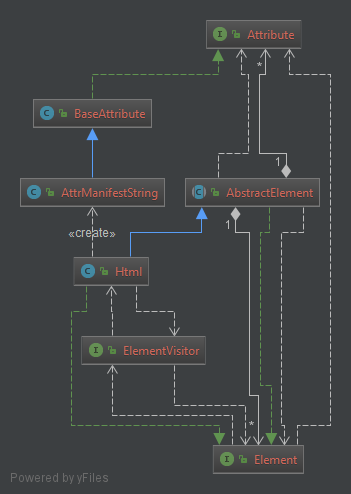
\includegraphics[width=1\textwidth]{infrastructure}
	\caption{Fluent Interfaces - The Supporting Infrastructure}
	\label{img:infrastructure}
\end{figure}

\subsection{Code Generation Strategy}
\label{sec:codegenerationstrategy}

As we already presented before in the Section \ref{sec:problemstatement}, this solution focus on how the code is organized instead of making complex code. All the methods present in the generated classes have very low complexity, mainly adding information to the element children or to the attribute list. To reduce repeated code many interfaces with default methods are created so different classes can implement them and reuse the code. The complexity of the generated code is mostly present in the \texttt{AbstractElement} class, which implements most of the \texttt{Element} interface methods. Another very important aspect of the generated classes is the extensive use of \textit{type arguments}, also known as generics, which allows the navigation in the element tree while maintaining type information, which is essential to guarantee the specific language restrictions.

\subsection{Type Parameters}
\label{sec:typeparameters}

As this solution was designed an objective became clear, the generated \textit{fluent interface} should be easily navigable. This is crucial to provide a good user experience while creating templates through the \texttt{xmlet} \textit{fluent interfaces}. There are two main aspects, the \textit{fluent interface} should be easily navigable and always implement the concrete language restrictions. We tackle this issue through the use of \textit{type parameters}, which allow us to keep track of the tree structure of the elements that are being created and keep adding elements, or moving up in the tree structure without loosing the type information of the parent. In Listing \ref{lst:typeargumentsexplicit} we can observe how the type arguments work. 

\bigskip

\lstset{language=Java, morekeywords={Html, Body, Div, Element, P, Header}}

\begin{minipage}{\linewidth}
\begin{lstlisting}[caption={Example of the Explicit Use of Type Arguments},captionpos=b,label={lst:typeargumentsexplicit}]
Html<Element> html = new Html<>();
Body<Html<Element>> body = html.body();
        
P<Header<Body<Html<Element>>>> p1 = body.header().p();
P<Div<Body<Html<Element>>>> p2 = body.div().p();
        
Header<Body<Html<Element>>> header = p1.__();
Div<Body<Html<Element>>> div = p2.__();
\end{lstlisting}
\end{minipage}

\noindent
When we create the \texttt{Html} element we should indicate that he has a parent, for consistency. Then, as we add elements such as \texttt{Body} we automatically return the recently created \texttt{Body} element, but with parent information that indicates that this \texttt{Body} instance is descendant of an \texttt{Html} element. After that, we create two distinct \texttt{P} elements, \texttt{p1}, which has an \texttt{Header} parent, and \texttt{p2}, which has a \texttt{Div} parent. This information is reflected in the type of both variables, in line 4 and 5 of Listing \ref{lst:typeargumentsexplicit} respectively. Lastly, we can invoke the \texttt{\_\_} method, line 7 and 8 of Listing \ref{lst:typeargumentsexplicit}, which returns the current element parent, and observe that each \texttt{P} instance returns its respective parent object, with the correct type.

\noindent
In the example presented in Listing \ref{lst:typeargumentsexplicit} the usage of the \textit{fluent interface} might seem to be excessive verbose to define a simple \ac{HTML} document. For specific purposes it might be needed to extract variables, but in the most common usage of the \textit{fluent interface}  the code should be similar to Listing \ref{lst:typeargumentshidden}.  

\bigskip

\lstset{language=Java, morekeywords={Html}}

\begin{minipage}{\linewidth}
\begin{lstlisting}[caption={Example of the Implicit Use of Type Arguments},captionpos=b,label={lst:typeargumentshidden}]
new Html<>()
    .body()
        .header()
            .p().__()
        .__()
        .div()
            .p().__();
\end{lstlisting}
\end{minipage}

\noindent
To provide a better understanding on how this works we need to showcase three distinct classes. First we have the \texttt{AbstractElement} class, Listing \ref{lst:abstractelement}, which is the class from where all classes generated based on a \ac{XSD} \texttt{xsd:element} derive. This class receives two \textit{type parameters}: 

\begin{itemize}
	\item \textbf{T} - Represents the type of the concrete element; 
	\item \textbf{Z} - Represents the type of the parent of the concrete element.
\end{itemize}	

\lstset{language=Java, morekeywords={AbstractElement, Element, T, Z}}

\noindent
In the \texttt{\_\_} method, shown in line 8 of Listing \ref{lst:abstractelement}, the parent of any deriving class is returned. The type information is kept since the method returns \texttt{Z}, the \textit{type parameter} that is the type of the parent of the deriving class, as shown in lines 7 and 8 of Listing \ref{lst:typeargumentsexplicit}.

\bigskip

\begin{minipage}{\linewidth}
\begin{lstlisting}[caption={AbstractElement Class Type Arguments},captionpos=b,label={lst:abstractelement}]
class AbstractElement<T extends Element, Z extends Element>
	protected Z parent;
	
    protected AbstractElement(Z parent) {
        this.parent = parent;
    }	
	
	public Z __() {
		return this.parent;
	}
	
	// (...)
}
\end{lstlisting}
\end{minipage}

\noindent
The second class is the \texttt{Table} class, which represents the \texttt{table} \ac{XSD} element present on the \ac{HTML} \textit{fluent interface} generated by \texttt{xmlet}. It has a single \textit{type parameter}, Z, which represents the type of its parent. It extends \texttt{AbstractElement} and therefore indicates that his type is \texttt{Table<Z>} and its parent type is \texttt{Z}. Any  interface implemented by a class generated from a \ac{XSD} \texttt{xsd:element}, such as the \texttt{Table} class, should receive the same type information as the \texttt{AbstractElement} class, as shown with \texttt{TableChoice0}. Regarding the \texttt{attrBorder} method, it indicates that it returns the exact same type, since it returns the \texttt{this} object, i.e. \texttt{Table<Z>}.

\bigskip

\lstset{language=Java, morekeywords={Table, Element, Z, AbstractElement, TableChoice0, EnumBorderType}}

\begin{minipage}{\linewidth}
\begin{lstlisting}[caption={Html Class Type Arguments},captionpos=b,label={lst:abstractelement}]
class Table<Z extends Element> extends AbstractElement<Html<Z>, Z>
                               implements TableChoice0<Html<Z>, Z>
    // (...)
    
    public Table<Z> attrBorder(EnumBorderType attrBorder) {
        // ...
    }
}
\end{lstlisting}
\end{minipage}

\noindent
As the third class we have the \texttt{TableChoice0} interface, which has methods for each kind of element that is allowed as children in \texttt{table} elements. It should receive the same \textit{type parameters} as \texttt{AbstractElement}. In the current case, if an instance of \texttt{Table<Element>} invokes the \texttt{tbody} method, line 2 of Listing \ref{lst:tablechoice}, the type returned would be \texttt{Tbody<Table<Element}\texttt{>}\texttt{>} since the \texttt{T} type of \texttt{TableChoice0} is \texttt{Table<Z>} when the type \texttt{Table} implements it.

\bigskip

\lstset{language=Java, morekeywords={Element, Z, Tbody, T, TableChoice0}}

\begin{minipage}{\linewidth}
\begin{lstlisting}[caption={TableChoice0 Interface Type Arguments},captionpos=b,label={lst:tablechoice}]
interface TableChoice0<T extends Element<T, Z>, Z extends Element> 		                                           extends Element<T, Z> {
    default Tbody<T> tbody() {
        // ...
    }
}
\end{lstlisting}
\end{minipage}

\subsection{Restriction Validation}
\label{sec:restrictionvalidation}

In the description of any given \ac{XSD} file there are many restrictions in the way the elements are contained within each other and which attributes are allowed. To reflect those restrictions to Java language there are two alternatives, validation in runtime or in compile time. This library tries to validate most of the restrictions in compile time, as shown above by the way classes are created. But some restrictions cannot be validated in compile time, an example of this is the following attribute with a restriction shown in Listing \ref{lst:restrictionexample}.

\bigskip

\lstset{
	language=XML,
	morekeywords={xs:schema, xs:element, xs:complexType, xs:attribute, xs:simpleType, xs:restriction, xs:maxLength, xs:minLength, xs:list}
}

\begin{minipage}{\linewidth}
\begin{lstlisting}[caption={Restrictions Example XSD},captionpos=b,label={lst:restrictionexample}]
<xs:schema>
    <xs:element name="testElement">
        <xs:complexType>
            <xs:attribute name="intList" type="valuelist"/>
        </xs:complexType>
    </xs:element>
    
    <xs:simpleType name="valuelist">
        <xs:restriction>
            <xs:maxLength value="5"/>
            <xs:minLength value="1"/>
        </xs:restriction>
        <xs:list itemType="xsd:int"/>
    </xs:simpleType>
</xs:schema>
\end{lstlisting}
\end{minipage}

\noindent
In this example, Listing \ref{lst:restrictionexample}, we have an element, i.e. \texttt{testElement} on line 2, which has an attribute called \texttt{intList}, on line 4. This attribute has some restrictions, it is represented by a \texttt{xs:list}, the list elements have the \texttt{xsd:int} type and its element count should be between 1 and 5, restriction element on line 9 of Listing \ref{lst:restrictionexample}. Transporting this example to the Java language will result in the following class shown on Listing \ref{lst:attributeclassexample}.

\bigskip

\lstset{language=Java, morekeywords={BaseAttribute, List, Integer, AttrIntList}}

\begin{minipage}{\linewidth}
\begin{lstlisting}[caption={Attribute Class Receiving a List},captionpos=b,label={lst:attributeclassexample}]
public class AttrIntList extends BaseAttribute<List<Integer>> {
    public AttrIntList(List<Integer> list) {
        super(list);
    }
}
\end{lstlisting}
\end{minipage}

\noindent
But with this solution the \texttt{xs:maxLength} and \texttt{xs:minLength} values are ignored. To solve this problem the existing restrictions in any given attribute are \textit{hardcoded} in the class constructor, which invokes methods present in the \texttt{RestrictionValidator} class that validate each type of restriction, e.g. \texttt{xs:maxLength} and \texttt{xs:minLength}. The values present in the restrictions on the \ac{XSD} document are \textit{hardcoded} in the \textit{bytecodes} and help validate each attribute object that is created. This results in the generation of a constructor as shown in Listing \ref{lst:attrhardcodedrestrictions}.

\bigskip

\lstset{language=Java, morekeywords={BaseAttribute, List, Integer, RestrictionValidator, AttrIntList}}

\begin{minipage}{\linewidth}
\begin{lstlisting}[caption={Attribute Constructor Enforcing Restrictions},captionpos=b,label={lst:attrhardcodedrestrictions}]
public class AttrIntList extends BaseAttribute<List<Integer>> {
    public AttrIntList(List<Integer> attrValue) {
        super(attrValue, "intlist");
        RestrictionValidator.validateMaxLength(5, attrValue);
        RestrictionValidator.validateMinLength(1, attrValue);
    }
}

\end{lstlisting}
\end{minipage}

\noindent
There are a total of thirteen different restrictions on the \ac{XSD} language. The \texttt{RestrictionValidator} class is a class with static methods that allow to validate most of those restrictions, the only restrictions that are not validated by this class are \texttt{xsd:enumeration} restrictions, which are already validated by the usage of \texttt{Enum} classes and \texttt{xsd:whitespace} since it represents an indication instead of an actual restriction on the language. In Listing \ref{lst:restrictionvalidator} we can observe how simple is to validate the \texttt{xs:maxLength} and \texttt{xs:minLength} restrictions that were used in the previous example. All the methods work in the exact same way, a condition is verified and if the verification fails it will throw a \texttt{RestrictionViolationException} with a message describing the nature of the violated restriction.

\bigskip

\lstset{language=Java, morekeywords={RestrictionValidator, RestrictionViolationException, List}}

\begin{minipage}{\linewidth}
\begin{lstlisting}[caption={RestrictionValidator Class - The Validation Methods},label={lst:restrictionvalidator}]
public class RestrictionValidator {
    public static void validateMaxLength(int maxLength, List list){
        if (list.size() > maxLength){
            throw new RestrictionViolationException("Violation of maxLength restriction");
        }
    }
    
    public static void validateMinLength(int minLength, List list){
        if (list.size() < minLength){
            throw new RestrictionViolationException("Violation of minLength restriction");
        }
    }
}
\end{lstlisting}
\end{minipage}

\subsubsection{Enumerations}
\label{sec:enumarations}

Regarding restrictions there is one that can be enforced at compile time, the \texttt{xs:enumeration}. To obtain that validation at compile time the XsdAsm library generates \texttt{Enum} classes that contain all the values indicated in the \texttt{xs:enumeration} elements. In the following example, Listing \ref{lst:enumxsddefinition}, we have an attribute with three possible values: \texttt{command}, \texttt{checkbox} and \texttt{radio}.

\bigskip

\lstset{language=XML, morekeywords={xs:attribute, xs:simpleType, xs:restriction, xs:enumeration}}

\begin{minipage}{\linewidth}
\begin{lstlisting}[caption={Example of an Enumeration in XSD Definition},label={lst:enumxsddefinition}]
<xs:attribute name="type">
    <xs:simpleType>
        <xs:restriction base="xsd:string">
            <xs:enumeration value="command" />
            <xs:enumeration value="checkbox" />
            <xs:enumeration value="radio" />
        </xs:restriction>
    </xs:simpleType>
</xs:attribute>
\end{lstlisting}
\end{minipage}

\noindent
This results in the creation of an \texttt{Enum} class, \texttt{EnumTypeCommand}, presented in Listing \ref{lst:enumclass}. The attribute class will then receive an instance of \texttt{EnumTypeCommand}, ensuring that only allowed values are used (Listing \ref{lst:enumusage}).

\bigskip

\lstset{language=Java, morekeywords={enum, String, EnumTypeCommand}}

\begin{minipage}{\linewidth}
\begin{lstlisting}[caption={Example of a Generated Enumeration Class},label={lst:enumclass}]
public enum EnumTypeCommand {
    COMMAND(String.valueOf("command")), 
    CHECKBOX(String.valueOf("checkbox")),
    RADIO(String.valueOf("radio"))
}
\end{lstlisting}
\end{minipage}

\lstset{language=Java, morekeywords={EnumTypeCommand, AttrTypeEnumTypeCommand, String, BaseAttribute}}

\begin{minipage}{\linewidth}
\begin{lstlisting}[caption={Attribute Receiving An Enumeration Instance},label={lst:enumusage}]
public class AttrTypeEnumTypeCommand extends BaseAttribute<String> {
    public AttrTypeEnumTypeCommand(EnumTypeCommand attrValue) {
        super(attrValue.getValue());
    }
}
\end{lstlisting}
\end{minipage}

\newpage

\subsection{Element Binding}
\label{sec:elementbinding}

\noindent
To support the definition of reusable templates the \texttt{Element} and \texttt{AbstractElement} classes were modified to support binders. This allows programmers to postpone the addition of information to the defined element tree. An example is presented in Listing \ref{lst:binderusage} using the \ac{HTML}5 \textit{fluent interface}.

\bigskip

\lstset{language=Java, morekeywords={BinderExample, Element, Html,  List, String}}

\begin{minipage}{\linewidth}
\begin{lstlisting}[caption={Binder Usage Example},label={lst:binderusage}]
public class BinderExample{
    public void bindExample(){
        Html<Element> root = new Html<>()
            .body()
                .table()
                    .tr()
                        .th()
                            .text("Title")
                        .__()
                    .__()
                    .<List<String>>binder((elem, list) ->
                         list.forEach(tdValue ->
                                 elem.tr().td().text(tdValue)
                         )
                    )
                .__()
            .__()
        .__();
    }
}
\end{lstlisting}
\end{minipage}

\noindent
In this example we use the \ac{HTML} language to create a document that contains a table with a title in the first row as a title header , i.e. \texttt{th()}. Regarding the values presented in the table, instead of having them inserted right away, it is possible to delay that insertion by postponing a function, as shown on line 11 of Listing \ref{lst:binderusage}, to be executed when the information is received, i.e. the \texttt{list} on line 11 of Listing \ref{lst:binderusage}. This is achieved by implementing an \texttt{ElementVisitor} that supports binding. 

\noindent
In Listing \ref{lst:visitorbinding} we can observe how an \texttt{ElementVisitor} implementation that supports binders would work, while maintaining the default behaviour for the elements that are not bound, i.e. \texttt{else} clause in line 16 of Listing \ref{lst:visitorbinding}. If the element is bound to a function this implementation will clone the element, i.e. the \texttt{cloneElem} function in line 12 of Listing \ref{lst:visitorbinding}, and apply a model to the cloned object, i.e. the model being a \texttt{List<String>} object following the example of shown Listing \ref{lst:binderusage}, effectively executing the function supplied in the previously shown \texttt{binder} method, i.e. line 11 of Listing \ref{lst:binderusage}. This function call will generate new children on the cloned \texttt{table} instance that will be iterated as if they belonged to the original element tree. This behaviour ensures that the original element tree is not affected since all these changes are performed in a clone of the bound element, meaning that the template can be reused.

\bigskip

\lstset{language=Java, morekeywords={CustomVisitor, T, List, Element, R}}

\begin{minipage}{\linewidth}
\begin{lstlisting}[caption={Visitor with Binding Support},label={lst:visitorbinding}]
public class CustomVisitor<R> implements ElementVisitor<R> {

   private R model;

   public CustomVisitor(R model){
       this.model = model;
   }
    
   public <T extends Element> void sharedVisit(Element<T,?> element) {
       // ...
       if(element.isBound()) {
           List<Element> children = element.cloneElem()
                                           .bindTo(model)
                                           .getChildren();
           children.forEach( child -> child.accept(this));
       } else {
           element.getChildren().forEach(item -> item.accept(this));
       }
       // ...
   }
}
\end{lstlisting}
\end{minipage}
        
\subsection{Using the Visitor Pattern}
\label{sec:xsdasmvisitor}

In the previous sections we presented how the \textit{fluent interface} is generated and how it implements the language restrictions, but what can the \textit{fluent interface} actually be used for? That is strictly up to the user of the generated \textit{fluent interface}. To achieve this we use the \texttt{Visitor} pattern\citep{gamma1994design}. There are multiple \texttt{visit} methods that are invoked by the generated classes and the user can define the behaviour for each one of them by creating a concrete implementation of the \texttt{ElementVisitor} class. This way the generated code delegates the responsibility of defining the output of the \texttt{fluent interface} usage. The generated \texttt{ElementVisitor} class defines four main \texttt{visit} methods, Listing \ref{lst:elementvisitorasm}:

\begin{itemize}
	\item \texttt{sharedVisit(Element<T, ?> element)} - This method is called whenever a class generated based on a \ac{XSD} \texttt{<xsd:element>} has its \texttt{accept} method called. By receiving the \texttt{Element} we have access to the element children and attributes.
	\item \texttt{visit(Text text)} - This method is called when the \texttt{accept} method of the special \texttt{Text} element is invoked.
	\item \texttt{visit(Comment comment)} - This method is called when the \texttt{accept} method of the special \texttt{Comment} element is invoked.
	\item \texttt{visit(TextFuction<R, U, ?> textFunction)} - This method is called when the \texttt{accept} method of the special \texttt{TextFunction} element is invoked.
\end{itemize}	

\bigskip

\lstset{language=Java, morekeywords={ElementVisitor, T, Element, Text, Comment, TextFunction, U, R}}

\begin{minipage}{\linewidth}
\begin{lstlisting}[caption={ElementVisitor Generated by XsdAsm - The Core Methods},label={lst:elementvisitorasm}]
public abstract class ElementVisitor<R> {
   <T extends Element> void sharedVisit(Element<T, ?> element);

   void visit(Text text);

   void visit(Comment comment);

   <U> void visit(TextFunction<R, U, ?> textFunction);
}
\end{lstlisting}
\end{minipage}

\noindent
Apart from these four main method we also create specific methods, as shown in Listing \ref{lst:elementvisitorasmspecific}. These methods default behaviour is to invoke the main \texttt{sharedVisit(Element<T, ?> element)} method, but they can be redefined to perform a different action, providing the option of having a very simple implementation of only four methods or redefine all the methods for a concrete purpose for the respective \ac{DSL}.

\bigskip

\lstset{language=Java, morekeywords={ElementVisitor, Html}}

\begin{minipage}{\linewidth}
\begin{lstlisting}[caption={ElementVisitor Generated by XsdAsm - The Specific Methods},label={lst:elementvisitorasmspecific}]
public abstract class ElementVisitor {
   // (...)

   default void visit(Html html) {
      this.sharedVisit(html);
   }
}
\end{lstlisting}
\end{minipage}

\subsection{Performance - XsdAsmFaster}
\label{sec:xsdasmfaster}

The \texttt{xmlet} developed two alternative solutions to generate \textit{fluent interfaces}. The first solution that was implemented was XsdAsm, which generated a \textit{fluent interface} that defined element and attribute classes. When interacting with those elements it was possible to add children or attributes that were stored in a data structure as seen by the implementation of \texttt{AbstractElement} and the snippet of the \texttt{Html} code present in Listing \ref{lst:abstractelementasm} and Listing \ref{lst:htmlasm}, respectively.

\bigskip

\lstset{language=Java, morekeywords={AbstractElement, Element, T, Z, List, Attribute, ArrayList, R}}

\begin{minipage}{\linewidth}
\begin{lstlisting}[caption={AbstractElement Class Generated by XsdAsm},label={lst:abstractelementasm}]
abstract class AbstractElement<T extends Element, Z extends Element> implements Element<T, Z> {
   protected List<Element> children = new ArrayList();
   protected List<Attribute> attrs = new ArrayList();
   // (...)

   public <R extends Element> R addChild(R child) {
      this.children.add(child);
      return child;
   }
   public T addAttr(Attribute attribute) {
      this.attrs.add(attribute);
      return this.self();
   }
}
\end{lstlisting}
\end{minipage}

\bigskip

\lstset{language=Java, morekeywords={Z, Element, AbstractElement, ElementVisitor, String, AttrManifest, Body, Head, Html}}

\begin{minipage}{\linewidth}
\begin{lstlisting}[caption={Html Class Generated by XsdAsm},label={lst:htmlasm}]
class Html<Z extends Element> extends AbstractElement<Html<Z>, Z> {
   public void accept(ElementVisitor visitor) { visitor.visit(this); }
   
   public Html<Z> attrManifest(String attrManifest) {
      return (Html)this.addAttr(new AttrManifestString(attrManifest));
   }
   
   public Body<T> body() { return this.addChild(new Body(this)); }
   
   public Head<T> head() { return this.addChild(new Head(this)); }
}
\end{lstlisting}
\end{minipage}

\noindent
By using the solution generated by XsdAsm we ended up with a \textit{fluent interface} that works in a two steps basis:

\begin{itemize}  
	\item Creating the \texttt{Element} tree - We need to create the element tree by adding all elements and attributes, as shown in Listing \ref{lst:treebuilding};
	\item Visiting the \texttt{Element} tree - We need to invoke the \texttt{accept} method of the root of the tree in order for the whole tree to be visited, as shown in Listing \ref{lst:treevisit}.
\end{itemize}

\bigskip

\lstset{language=Java, morekeywords={Html}}

\begin{minipage}{\linewidth}
\begin{lstlisting}[caption={HTML5 Tree Creation using XsdAsm},label={lst:treebuilding}]
Html<Html> root = new Html<>();

root.head()
        .title()
            .text("Title")
        .__()
    .__()
    .body().attrClass("clear")
        .div()
        	.h1()
        		.text("H1 text")
        	.__()
        .__()
    .__()
.__();
\end{lstlisting}
\end{minipage}

\lstset{language=Java, morekeywords={CustomVisitor}}

\begin{minipage}{\linewidth}
\begin{lstlisting}[caption={HTML5 Tree Visit using XsdAsm},label={lst:treevisit}]
CustomVisitor customVisitor = new CustomVisitor();
// root variable created in the previous Listing.
root.accept(customVisitor);
\end{lstlisting}
\end{minipage}

\noindent
Even though that this solution worked fine it had a performance issue. Why were we adding elements to a data structure just for it to be iterated at a later time? From this idea a new solution was born, XsdAsmFaster. This new solution aims to perform the same operations, faster, while providing a very similar user experience to the \textit{fluent interface} generated by XsdAsm. To achieve that instead of storing information on a data structure we directly invoke the \texttt{ElementVisitor visit} method, this removes the need of storing and iterating information while maintaining all the expected behaviour. The two main moments that are affected by this change are the moments when an element is added to the tree and when an attribute is added to a previously created element. The code generated by XsdAsmFaster to add elements is as shown in Listing \ref{lst:htmlxsdasmfaster}.

\lstset{language=Java, morekeywords={Html, Z, Element, ElementVisitor, String, Body, T, Head}}

\begin{minipage}{\linewidth}
\begin{lstlisting}[caption={Html Class Generated by XsdAsmFaster},label={lst:htmlxsdasmfaster}]
public final class Html<Z extends Element> {
   protected final Z parent;
   protected final ElementVisitor visitor;

   public Html(ElementVisitor visitor) {
      this.visitor = visitor;
      visitor.visitElementHtml(this);
   }

   public Html(Z parent) {
      this.parent = parent;
      this.visitor = parent.getVisitor();
      this.visitor.visitElementHtml(this);
   }
   
   public final Html<Z> attrManifest(String attrManifest) {
      this.visitor.visitAttributeManifest(attrManifest);
      return this;
   }
   
   public Body<T> body() { return new Body(this); }
   public Head<T> head() { return new Head(this); }
}
\end{lstlisting}
\end{minipage}

\noindent
As we can see in Listing \ref{lst:htmlxsdasmfaster} we can invoke the \texttt{visit} method in the constructor of the classes generated based on a \ac{XSD} \texttt{<xsd:element>}, such as \texttt{Html} or \texttt{Body}, since the \texttt{ElementVisitor} instance is accessible for all the elements on the element tree. Since adding elements results in the creation of new objects, such as \texttt{Body} and \texttt{Head} in lines 22 and 24 of Listing \ref{lst:htmlxsdasmfaster} respectively, it results in the invocation of their respective \texttt{visit} method due to the \texttt{visit} method being called in each class constructor. The attributes have a very similar behaviour, although they do not have instances created their restrictions are validated by invoking a static validate method present in each attribute class. If the attribute has no restrictions then the behaviour is as shown in Listing \ref{lst:htmlxsdasmfaster}, where the respective \texttt{visit} method is called the method ends returns the object \texttt{this} to continue with the fluent tree creation.

\noindent
The XsdAsmFaster solution also adds many other performance improvements. The \texttt{ElementVisitor} methods were changed to receive \texttt{String} objects instead of \texttt{Attribute} types. Changing this removes the requirement to instantiate attribute classes since we can directly pass the \texttt{name} of the attribute and its \texttt{value} as shown in \texttt{attrManifest} method in Listing \ref{lst:htmlxsdasmfaster}. This change was performed since the only contained fields in attribute classes were \texttt{name} and \texttt{value}. The \texttt{ElementVisitor} class of XsdAsmFaster is as present in Listing \ref{lst:elementvisitorxsdasmfaster}.

\bigskip

\lstset{language=Java, morekeywords={ElementVisitor, String, R, Element, Text, Html}}

\begin{minipage}{\linewidth}
\begin{lstlisting}[caption={ElementVisitor Generated by XsdAsmFaster},label={lst:elementvisitorxsdasmfaster}]
public abstract class ElementVisitor {
   public abstract void visitElement(Element element);
   public abstract void visitAttribute(String attributeName, 
                                       String attributeValue);
   public abstract void visitParent(Element element);
   public abstract <R> void visitText(Text<? extends Element, R> t);
   public abstract <R> void visitComment(Text<? extends Element, R> t);

   public void visitOpenDynamic() {   }
   public void visitCloseDynamic() {   }

   // The methods below are generated based on the generated elements.
   public void visitParentHtml(Html element) {
      this.visitParent(element);
   }
   public void visitElementHtml(Html element) {
      this.visitElement(element);
   }
}
\end{lstlisting}
\end{minipage}

\noindent
Another feature that was introduced with XsdAsmFaster is both methods \texttt{visitOpenDynamic} and \texttt{visitCloseDynamic}. These methods have the objective to inform the concrete implementation of the \texttt{ElementVisitor} type that every \texttt{visit} method called in between calls of \texttt{visitOpenDynamic} and \texttt{visitCloseDynamic} represent dynamic data. That also means that every other \texttt{visit} method call outside of the dynamic spectrum is static. In Section \ref{sec:htmlflow3} we will show how this feature can be used to improve the performance of the resulting solution.

\newpage

\section{Client} % (fold)
\label{sec:client}

To use and test both \hyperref[sec:xsdasm]{XsdAsm} and \hyperref[sec:xsdparser]{XsdParser} we needed to implement a client for XsdAsm. Three different clients were implemented, one using the \ac{HTML}5 specification, one using the specification for Android visual layouts and another one by creating a specification for the regular expression language. In this section we are going to explore how the \ac{HTML}5 \textit{fluent interface} is generated using the XsdAsm library and how to use it. Other generated \textit{fluent interfaces}, such as the Android Layouts and Regex, follow the exact same process in their creation and usage.

\subsection{HtmlApi}
\label{sec:htmlapi}

To generate the \ac{HTML}5 \textit{fluent interface} we need to obtain its \ac{XSD} file. After that there are two options, the first one is to create a Java project that invokes the XsdAsm \texttt{main} method directly by passing the path of the specification file and the desired \textit{fluent interface} name that will be used to create a custom package name, shown in Listing \ref{lst:directapicreation}.

\bigskip

\lstset{language=Java, morekeywords={XsdAsmMain, String}}

\begin{minipage}{\linewidth}
\begin{lstlisting}[caption={Fluent Interface Creation},label={lst:directapicreation}]
void generateApi(String xsdFilePath, String apiName){
    XsdAsmMain.main(new String[] {xsdFilePath, apiName} );    
}
\end{lstlisting}
\end{minipage}

\noindent
The second option is using the Maven\cite{maven} build lifecycle\cite{mavenlifecycle} to make that same invocation by adding an extra execution to the \ac{POM} file, shown in Listing \ref{lst:mavencreation}, to execute a batch file that invokes the XsdAsm \texttt{main} method, shown in Listing \ref{lst:creationbat}. More information about Maven will be provided in Section \ref{sec:maven}.

\bigskip

\lstset{language=XML, morekeywords={plugin, artifactId, groupId, executions, execution, id, phase, goals, goal, configuration, executable, basedir}}

\begin{minipage}{\linewidth}
\begin{lstlisting}[caption={Maven - Compiling Classes using a Plugin},label={lst:mavencreation}]
<plugin>
    <artifactId>exec-maven-plugin</artifactId>
    <groupId>org.codehaus.mojo</groupId>
    <version>1.6.0</version>
    <executions>
        <execution>
            <id>create_classes1</id>
            <phase>validate</phase>
            <goals>
                <goal>exec</goal>
            </goals>
            <configuration>
                <executable>
                    ${basedir}/create_class_binaries.bat
                </executable>
            </configuration>
        </execution>
    </executions>
</plugin>
\end{lstlisting}
\end{minipage}

\lstset{language=bash, morekeywords={exist, not, call, mvn, java, mkdir, rmdir}}

\begin{minipage}{\linewidth}
\begin{lstlisting}[caption={Maven - The Code that creates the Fluent Interface Classes (create\_class\_binaries.bat)},label={lst:creationbat}]
if exist "./src/main/java" rmdir "./src/main/java" /s /q

if not exist "./target/classes/org/xmlet/htmlapi" 
    mkdir "./target/classes/org/xmlet/htmlapi"

call 
    mvn exec:java -D"exec.mainClass"="org.xmlet.xsdasm.main.XsdAsmMain" 
    -D"exec.args"="./src/main/resources/html_5.xsd htmlapi"
\end{lstlisting}
\end{minipage}

\noindent
This client uses the Maven lifecycle option by adding an execution at the \texttt{validate} phase, shown in line 8 of Listing \ref{lst:mavencreation}, which invokes XsdAsm \texttt{main} method to create the \textit{fluent interface}. This invocation of XsdAsm creates all the classes in the target folder of the HtmlApi project. Following these steps would be enough to allow any other Maven project to add a dependency to the HtmlApi project and use its generated classes as if they were manually created. But this way the source files and Java documentation files are not created since XsdAsm only generates the class binaries. To tackle this issue we added another execution to the \ac{POM}. This execution uses the Fernflower\cite{fernflower} decompiler, the Java decompiler used by Intellij\cite{intellij} \ac{IDE}, to decompile the classes that were automatically generated, shown in Listing \ref{lst:mavendecompilation} and Listing \ref{lst:decompilationbat}.

\bigskip

\lstset{language=XML, morekeywords={plugin, artifactId, groupId, executions, execution, id, phase, goals, goal, configuration, executable, basedir}}

\begin{minipage}{\linewidth}
\begin{lstlisting}[caption={Maven - Decompiling Classes Using the Fernflower Plugin},label={lst:mavendecompilation}]
<execution>
    <id>decompile_classes</id>
    <phase>validate</phase>
    <goals>
        <goal>
            exec
        </goal>
    </goals>
    <configuration>
        <executable>
            ${basedir}/decompile_class_binaries.bat
        </executable>
    </configuration>
</execution>
\end{lstlisting}
\end{minipage}

\lstset{language=bash, morekeywords={exist, not, call, mvn, java, mkdir, rmdir}}

\begin{minipage}{\linewidth}
\begin{lstlisting}[caption={Maven - The Code to Decompile the Generated Classes (decompile\_class\_binaries.bat)},label={lst:decompilationbat}]
if not exist "./src/main/java/org/xmlet/htmlapi" mkdir "./src/main/java/org/xmlet/htmlapi"

call 
    mvn exec:java 
    -D"exec.mainClass"="org.jetbrains.java.decompiler.main.decompiler.ConsoleDecompiler" 
    -D"exec.args"="-dgs=true ./target/classes/org/xmlet/htmlapi ./src/main/java/org/xmlet/htmlapi"

if exist "./target/classes/org" rmdir "./target/classes/org" /s /q
\end{lstlisting}
\end{minipage}

\noindent
By decompiling those classes we obtain the source code, which allows us to delete the automatic generated classes and allow the Maven build process to perform the normal compiling process, which generates the Java documentation files and the class binaries, along with the source files obtained from the decompilation process. This process, apart from generating more information to the programmer that will use the \textit{fluent interface} in the future, also allows to find any problem with the generated code since it forces the compilation of all the classes previously generated.

\subsection{Using the HtmlApi}

After the previously described compilation process of the HtmlApi project we are ready to use the generated \textit{fluent interface}. To start using it the first step is to implement the \texttt{ElementVisitor} class, which defines what to do when the created element tree is visited. A very simple example is presented in Listing \ref{lst:customvisitorexample}, which writes the \ac{HTML} tags based on the name of the element type visited, i.e. the opening tag in line 8 and the closing tag on line 19 of Listing \ref{lst:customvisitorexample}, and navigates in the element tree by accessing the children of the current element type, i.e. the \texttt{getChildren()} method call followed by the invocation of the \texttt{accept} method call of every child present in the current element.

\bigskip

\lstset{language=Java, morekeywords={CustomVisitor, PrintStream, Element, T, ElementVisitor}}

\begin{minipage}{\linewidth}
\begin{lstlisting}[caption={Custom Visitor Example that Implements the ElementVisitor Generated by XsdAsm},label={lst:customvisitorexample}]
public class CustomVisitor<R> implements ElementVisitor<R> {

   private PrintStream printStream = System.out;

   public CustomVisitor(){ }

   public <T extends Element> void sharedVisit(Element<T,?> element) {
       printStream.printf("<%s", element.getName());

       element.getAttributes()
              .forEach(attribute -> 
                  printStream.printf(" %s=\"%s\"", 
                      attribute.getName(), attribute.getValue()));

       printStream.print(">\n");

       element.getChildren().forEach(item -> item.accept(this));

       printStream.printf("</%s>\n", element.getName());
   }
}
\end{lstlisting}
\end{minipage}

\newpage

\noindent
After creating the \texttt{CustomVisitor} presented in Listing \ref{lst:customvisitorexample} we can start to create the element tree of the document that we want to present. To start we should create a \texttt{Html} object, since all the \ac{HTML} documents have it as a base element. Upon creating that root element we can start to add other elements or attributes that will appear as options based on the specification rules. To help with the navigation on the element tree a method was created to allow the navigation to the parent of any given element. This method is named \texttt{\_\_}, a short method name to keep the code as clean as possible. In Listing \ref{lst:htmlapicodeexample} we can see a code example that uses a good amount of the \textit{fluent interface} features:

\begin{itemize}
	\item Element creation - For example, the \texttt{root.head()} method call adds an \texttt{Head} instance to the \texttt{Html} root element;
	\item Attribute assignment - For example, the \texttt{body().attrClass("clear")} method call adds the attribute \texttt{class} with the value \texttt{clear} to the \texttt{Body} instance created with the \texttt{body()} method call;
	\item Attributes receiving \texttt{Enum} classes - The \texttt{attrType(EnumTypeContentType.TEXT\_CSS)} call, which indicates that the type value should be \texttt{text/css}, which is the value present in \texttt{EnumTypeContentType.TEXT\_CSS};
	\item Parent navigation - Both \texttt(\_\_()) method calls at the end of line 10 of Listing \ref{lst:htmlapicodeexample} will result in the current context being changed from the \texttt{Link} type to the \texttt{Head} type by the first call, followed by another call with changes the context from the \texttt{Head} type to the \texttt{Html} type. This allows to proceed with the definition of the \texttt{Body} type, which can only be contained in the \texttt{Html} type.
\end{itemize}

\bigskip
\lstset{language=Java, morekeywords={Html, EnumTypeContentType, CustomVisitor}}

\begin{minipage}{\linewidth}
\begin{lstlisting}[caption={HtmlApi - The Definition of the Element Tree},label={lst:htmlapicodeexample}]
Html<Html> root = new Html<>();

root.head()
        .meta().attrCharset("UTF-8").__()
        .title()
            .text("Title").__()
        .link().attrType(EnumTypeContentType.TEXT_CSS)
               .attrHref("/assets/images/favicon.png").__()
        .link().attrType(EnumTypeContentType.TEXT_CSS)
               .attrHref("/assets/styles/main.css").__().__()
     .body().attrClass("clear")
        .div()
            .header()
                .section()
                    .div()
                        .img().attrId("brand")
                              .attrSrc("./assets/images/logo.png").__()
                        .aside()
                            .em()
                                .text("Advertisement")
                            .span()
                                .text("HtmlApi is great!");
                                    
CustomVisitor customVisitor = new CustomVisitor();
    
customVisitor.visit(root);
\end{lstlisting}
\end{minipage}

\noindent
With this element tree presented in Listing \ref{lst:htmlapicodeexample} and the previously presented \texttt{CustomVisitor}, shown in Listing \ref{lst:customvisitorexample}, we obtain the following result as shown in Listing \ref{lst:htmlapiresult}. The indentation was added for readability purposes, since the \texttt{CustomVisitor} implementation in Listing \ref{lst:customvisitorexample} does not indent the resulting \ac{HTML}.

\bigskip

\lstset{language=html, morekeywords={header, section, aside}}

\begin{minipage}{\linewidth}
\begin{lstlisting}[caption={HtmlApi - The Result of the Element Tree Visit},label={lst:htmlapiresult}]
<html>
    <head>
        <meta charset="UTF-8">
        </meta>
        <title>
            Title
        </title>
        <link type="text/css" href="/assets/images/favicon.png">
        </link>
        <link type="text/css" href="/assets/styles/main.css">
        </link>
    </head>
    <body class="clear">
        <div>
            <header>
                <section>
                    <div>
                        <img id="brand" src="./assets/images/logo.png">
                        </img>
                        <aside>
                            <em>
                                Advertisement
                                <span>
                                    HtmlApi is great!
                                </span>
                            </em>
                        </aside>
                    </div>
                </section>
            </header>
        </div>
    </body>
</html>                          
\end{lstlisting}
\end{minipage}

\noindent
The \texttt{CustomVisitor} of Listing \ref{lst:htmlapiresult} is a very minimalist implementation since it does not indent the resulting \ac{HTML}, does not simplify elements with no children (i.e. the \texttt{link}/\texttt{img} elements) and other aspects that are particular to \ac{HTML} syntax. That is where the HtmlFlow library comes in, it implements the particular aspects of the \ac{HTML} syntax in its \texttt{ElementVisitor} implementation that deals with how and where the output is written.

\subsection{HtmlFlow 3}
\label{sec:htmlflow3}

The HtmlFlow 3 library suffered some significant changes from its first version. At the moment it defines two ways of defining templates, a \texttt{StaticView} type, which allows the creation of template that does not receive any input data, and a \texttt{DynamicHtml} type, which receives a Java function that defines the template. We have already presented some code examples of both types along this document, but here we are going to analyze them. For the \texttt{StaticHtml} we have Listing \ref{lst:htmlflowstaticview}, which is the same as Listing \ref{lst:staticview}, duplicated here for explanation purposes.

\bigskip

\lstset{language=java, morekeywords={StaticHtml}}

\begin{minipage}{\linewidth}
\begin{lstlisting}[caption={HtmlFlow - Static View Example}, label={lst:htmlflowstaticview}]
private static void staticView(StaticHtml view){
    view.html()
            .body()
                .h1()
                    .text("This is a static view h1 element.")
                .__()
            .__()
        .__();
}
\end{lstlisting}
\end{minipage} 

\noindent
With the definition of this template, i.e. Listing \ref{lst:htmlflowstaticview}, we observe that this is a straightforward template, it has a couple of elements and does not require any external input. This type of template can be defined with any function that returns \texttt{void} and receives a \texttt{StaticView} object, i.e. a \texttt{Consumer<StaticView>} object.

\bigskip

\lstset{language=java, morekeywords={String, DynamicHtml, CurrentClass, Student}}

\begin{minipage}{\linewidth}
\begin{lstlisting}[caption={HtmlFlow - Xmlet Template with Student Information}, label={lst:htmlflowxmletdynamicstudentinfo}]
String document = DynamicHtml.view(CurrentClass::studentView)
                             .render(new Student("Luis", 39378));

static void studentView(DynamicHtml<Student> view, Student student){
    view.html()
          .body()
            .ul()
              .li().dynamic(li -> li.text(student.getName())).__()
              .li().dynamic(li -> li.text(student.getNumber())).__()
            .__()
          .__()
        .__();   
}
\end{lstlisting}
\end{minipage} 

\noindent
Regarding \texttt{DynamicHtml} templates, we can use and define them as shown in Listing \ref{lst:htmlflowxmletdynamicstudentinfo}. Their use is very similar, but there are a few noticeable changes. The first one is that now the function that is defining the template receives the \textit{context object} associated with the template, which in Listing \ref{lst:htmlflowxmletdynamicstudentinfo} is a \texttt{Student} object. The second change is that now the template should use a function, \texttt{dynamic} in lines 8 and 9 of Listing \ref{lst:htmlflowxmletdynamicstudentinfo}, to input dynamic information in the defined template while in the \texttt{StaticHtml} there was not such a call. This \texttt{dynamic} method has a very important significance in HtmlFlow 3, it provides information that the actions that will be performed inside the \texttt{Consumer} used as its parameter are dynamic and are subject to changes depending on the input received. Through the invocation of this method and thanks to strategy implemented by HtmlApiFaster the HtmlFlow 3 library has enough information to implement a caching strategy. In Listing \ref{lst:dynamicmethod} we can observe how HtmlApiFaster defines its \texttt{dynamic} methods, and how it notifies the \texttt{ElementVisitor} instance of the start, i.e. the invocation of \texttt{visitOpenDynamic()} method, and the end, i.e. the invocation of \texttt{visitCloseDynamic()} method, of the dynamic block.

\bigskip

\lstset{language=Java, morekeywords={Element, Z, ElementVisitor, Consumer, Li}}

\begin{minipage}{\linewidth}
\begin{lstlisting}[caption={Li Class - The dynamic method},label={lst:dynamicmethod}]
public final class Li<Z extends Element> {

   private ElementVisitor visitor;

   public Li<Z> dynamic(Consumer<Li<Z>> consumer){
      visitor.visitOpenDynamic();
      consumer.accept(this);
      visitor.visitCloseDynamic();
      return this;
   }   
}
\end{lstlisting}
\end{minipage}

\noindent
The caching strategy of HtmlFlow 3 uses a simple assumption, every action performed on the template elements that is not inserted in a dynamic block, i.e. is not performed inside of the \texttt{Consumer} used as a parameter to the \texttt{dynamic} method, is static information. This means that HtmlFlow 3 has sufficient information to cache different components of the template, e.g. in Listing \ref{lst:htmlflowxmletdynamicstudentinfo} HtmlFlow can store three components of the template: 

\begin{itemize}
	\item The \texttt{String} representing the \ac{HTML} text representing every element and attribute created before the call to the first \texttt{dynamic} method;
	\item The \texttt{String} representing the \ac{HTML} text representing every element and attribute created between the call to the first \texttt{dynamic} and second \texttt{dynamic} methods;
	\item The \texttt{String} representing the \ac{HTML} text representing every element and attribute created after the call to the second \texttt{dynamic} method;
\end{itemize}

\noindent
This greatly improves the performance of the solution. Without this caching strategy the library would perform many more \texttt{StringBuilder} operations, since the result of creating elements, adding attributes or closing elements in this particular implementation of the \texttt{ElementVisitor} type of the HtmlApiFaster \textit{fluent interface} is to use a \texttt{StringBuilder} object to \texttt{append} multiple \texttt{Strings}, added with the execution of the \texttt{visit} methods. By using the caching strategy the HtmlFlow 3 library avoids the invocation of the \texttt{append} method multiple times, which is decisive when it comes to performance.

\noindent
This version of the HtmlFlow library also supports another interesting feature, partial views. This feature is present in many \textit{template engines} since it allows for the same template to be used in many other templates, avoiding repetition. In Listing \ref{lst:htmlflowpartialviews} we present a simplified example that uses partial views. We have the presented method, i.e. \texttt{presentationsView}, which defines a template that receives multiple \texttt{Presentation} instances to present. Instead of defining the whole template, it uses another template that is responsible for specifying how a single \texttt{Presentation} instance is presented. In line 5 of Listing \ref{lst:htmlflowpartialviews} we can see how that works, we iterate the received \texttt{Iterable<Presentation> presentations} object and for each one of the objects we invoke the \texttt{addPartial} method, which receives the partial view instance, i.e. \texttt{PresentationView.view}, and the object that should be used to create the partial view.

\bigskip

\lstset{language=Java, morekeywords={DynamicHtml, Iterable, Presentation, PresentationView}}

\begin{minipage}{\linewidth}
\begin{lstlisting}[caption={HtmlFlow Partial Views},label={lst:htmlflowpartialviews}]
private static void presentationsView(DynamicHtml<Iterable<Presentation>> view, Iterable<Presentation> presentations){
    view.html()
            .body()
                .div()
                    .dynamic(div -> presentations.forEach(presentation -> view.addPartial(PresentationView.view, presentation)))
                .__()
            .__()
        .__();
}
\end{lstlisting}
\end{minipage}